\documentclass{beamer}

\usepackage{tikz}
\usepackage[labelfont=bf]{caption}
\usepackage{booktabs}
\usepackage{caption}
\usepackage{siunitx}
\usepackage{amsmath}
\usepackage{pgfplots}
\usepackage{pgfplotstable}

\title{Proving Conservation of Momentum through Relating Collision Outcomes}
\author{Henry Oehlrich\and Chelsea Liao\and Gra ce Jiang}

\begin{document}
\maketitle

\begin{frame}
    \frametitle{Abstract}
\end{frame}

\begin{frame}
    \frametitle{Experiment Setup}
    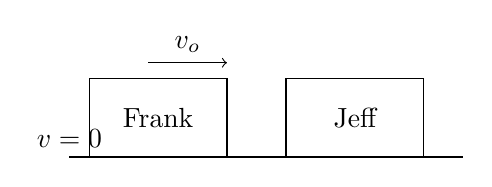
\begin{tikzpicture}
        \draw[thick] (0,0) -- (5,0);
        \draw[rectangle,color=black] (0.25,0) rectangle ++(1.75,1) node[midway] {Frank};
        \draw[->] (1,1.2) -> (2,1.2) node [midway,above] {$v_o$};
        \draw[rectangle,color=black] (2.75,0) rectangle ++(1.75,1) node[midway] {Jeff};
        \path (2.75,1) ++(1.75,0) node[midway,above] {$v=0$};
    \end{tikzpicture}
\end{frame}

\begin{frame}
    \frametitle{Materials and Methods}
\end{frame}

\begin{frame} 
    \frametitle{Results} 
\end{frame}

\begin{frame}
    \frametitle{Energy Relationship Graph}
\end{frame}

\begin{frame}
    \frametitle{Discussion}
\end{frame}

\end{document}
